%%%%%%%%%%%%%%%%%%%%%%%%%%%%%%%%%%%%%
% Inlucudings:                      %
%%%%%%%%%%%%%%%%%%%%%%%%%%%%%%%%%{{{%
\documentclass[11pt,english,a4paper,chapterprefix]{scrartcl}
\usepackage[T1]{fontenc}
\usepackage[bigcaptions]{listing}
\usepackage[utf8]{inputenc}
\usepackage[small,bf,hang]{caption}
\usepackage[english]{babel}
%\usepackage{epsfig}
\usepackage{wrapfig}
%\usepackage{caption}
\usepackage{psfrag}
\usepackage[rflt]{floatflt}
\usepackage[usenames]{color}
\usepackage{graphicx}
\emergencystretch = 10pt
\usepackage{amsmath}
\usepackage{amssymb}
\usepackage{setspace}
\usepackage{algpseudocode}
\usepackage{listing}
\usepackage{listings}
\usepackage{trsym}
\usepackage{trfsigns}
\usepackage{minted}
\usepackage{dirtree}
\setcounter{secnumdepth}{5}
\setcounter{tocdepth}{5} 
\numberwithin{equation}{section}
\numberwithin{figure}{section}

%%%%%%%%%%%%%%%%%%%%%%%%%%%%%%%%%}}}%
% New Commands and Configurations:  %
%%%%%%%%%%%%%%%%%%%%%%%%%%%%%%%%%{{{%
%\setkomafont{section}{\Large\rmfamily}
%\setkomafont{subsection}{\large\rmfamily}
%\setkomafont{subsubsection}{\normalsize\rmfamily}
\setkomafont{paragraph}{\footnotesize}
\numberwithin{table}{section}
\numberwithin{listing}{section}
\setlength\textheight{24cm}
\definecolor{orange}{rgb}{1 , 0.5 , 0}
\definecolor{blue}{rgb}{0, 0 , 1}
\definecolor{green}{rgb}{0, 1 ,0}
\newcommand{\cb}{\textcolor{blue}}
\newcommand{\subsubsubsection}{\paragraph}
\newcommand{\subsubsubsubsection}{\subparagraph}
\clubpenalty = 10000
\widowpenalty = 10000
\displaywidowpenalty = 10000
\parindent0pt % No Indent
\setlength{\parskip}{1em}
%\makenomenclature
% Document Head
\begin{document}
%\restylefloat{figure}
%\pagestyle{fancy}
%\rhead{} 

\definecolor{light-gray}{gray}{0.90}

\newminted{perl}{linenos, bgcolor=light-gray, fontsize=\scriptsize}
\newminted{cpp}{bgcolor=light-gray, fontsize=\scriptsize}
\newminted{tcl}{bgcolor=light-gray, fontsize=\scriptsize}
\newminted{sh}{bgcolor=light-gray, fontsize=\scriptsize}
\newminted{basemake}{bgcolor=light-gray, fontsize=\scriptsize}

%%%%%%%%%%%%%%%%%%%%%%%%%%%%%%%%%}}}%
% fancy nomenclautur:
%%%%%%%%%%%%%%%%%%%%%%%%%%%%%%%%%{{{%
%\setlength{\nomlabelwidth}{.20\hsize}
%\renewcommand{\nomlabel}[1]{#1 \dotfill}

%<*sample05>
\def\@@@nomenclature[#1]#2#3{%
 \def\@tempa{#2}\def\@tempb{#3}%
 \protected@write\@nomenclaturefile{}%
  {\string\nomenclatureentry{#1\nom@verb\@tempa @[{\nom@verb\@tempa}]%
    |nompageref{\begingroup\nom@verb\@tempb\protect\nomeqref{\theequation}}}%
    {\thepage}}%
 \endgroup
 \@esphack}
%\def\nompageref#1#2{%
%  \if@printpageref\pagedeclaration{#2}\else\null\fi
%  \linebreak#1\nomentryend\endgroup}
\def\pagedeclaration#1{\dotfill\nobreakspace ~#1}
%\def\nomentryend{.}
\def\nomlabel#1{\textbf{#1}\hfil}
\makeatletter 
\renewcommand*\dotfill{\leavevmode% 
  \leaders\hbox{$\m@th 
  \mkern \@dotsep mu\hbox{.}\mkern \@dotsep 
  mu$}\hfill\kern\z@} 
\makeatother
%%%%%%%%%%%%%%%%%%%%%%%%%%%%%%%%%}}}%
% Abbr Commands!
%%%%%%%%%%%%%%%%%%%%%%%%%%%%%%%%%{{{%
\newcommand{\abbr}[2]{\textit{#2} (#1)\nomenclature{#1}{#2 \nomrefpage}}
\newcommand{\shortabbr}[2]{\nomenclature{#1}{#2 \nomrefpage}}
\newcommand{\revabbr}[2]{#1 (\textit{#2})\nomenclature{#1}{#2 \nomrefpage}}

%%%%%%%%%%%%%%%%%%%%%%%%%%%%%%%%%}}}%
% Titlepage                         %
%%%%%%%%%%%%%%%%%%%%%%%%%%%%%%%%%{{{%
%%%%%%%%%%%%%%%%%%%%%%%%%%%%%%%%%%%%%%%%%%%%%%%%%%%%%%%%%%%%%%%%%%%%%%%%%%%%%%%%%%%%%%%%%%%%%%%%%%%
\begin{titlepage}
\setcounter{page}{-1}
\begin{center}

%\includegraphics*[scale=2.5]{img/TUKL_LOGO.pdf}\\[3ex]

%\textsc{\Large University of Kaiserslautern}\\[1.5ex]
%Department of Electrical Engineering and Information Technology\\[1.5ex]
%Microelectronic Systems Design Research Group \\[3ex]

\vfill
\vfill

\textsc{\Huge TTool-AMS}\\[6ex]
\centerline{\Large Integration of SystemC-AMS Simulation Platforms into TTool}
\vspace{20pt}

\vfill
\vfill

 \begin{tabular}{rl}\hline\\
         Author:                   & \quad Rodrigo Cortés Porto (University of Kaiserslautern) \\[1.5ex]
 Co-Authors:                    & \quad Dr. D. Genius (Sorbonne University, LIP6)\\[1.5ex]
 & \quad Irina Lee (Sorbonne University, Master SESI)\\[1.5ex]
                            & \quad Prof. L. Apvrille (Télécom Paris) \\[1.5ex]\\\hline
 \end{tabular}
\end{center}
 
%%%%%%%%%%%%%%%%%%%%%%%%%%%%%%%%%}}}%
    
\end{titlepage}


\newpage
%%%%%%%%%%%%%%%%%%%%%%%%%%%%%%%%%}}}%
% Table of Contents                 %
%%%%%%%%%%%%%%%%%%%%%%%%%%%%%%%%%{{{%
\tableofcontents
\thispagestyle{empty}
\addtocontents{toc}{\protect\thispagestyle{empty}}
\newpage
\setcounter{page}{1}
\newpage
%\setcounter{page}{1}
%%%%%%%%%%%%%%%%%%%%%%%%%%%%%%%%%}}}%
% Chapters                          %
%%%%%%%%%%%%%%%%%%%%%%%%%%%%%%%%%{{{%



\newpage
\clearpage

%clear headers
%\fancyhead{}
%\fancyfoot{}
%\fancyfoot[CO, CE] {\thepage}

%\setcounter{secnumdepth}{0}
%\begin{appendix}

\setcounter{section}{0}
%\renewcommand{\thesection}{\Alph{section}}
%\newcounter{AppendixCounter}
%\setcounter{AppendixCounter}{1}
%\renewcommand{\theAppendixCounter}{\Alph{AppendixCounter}}
%\phantomsection
%\addcontentsline{toc}{section}{Appendix~\theAppendixCounter: Source codes}
%\section*{Appendix~\theAppendixCounter: Source codes}

\section{Getting started}

\subsection{Virtual Machine}

In the \textit{Virtual Machine} version, tested under VirtualBox, TTool, as well as SoClib and MutekH
%and SystemC-AMS 
are preinstalled.
You will require to fetch SystemC-AMS from the Accelera website, which requires registration:

\texttt{www.accellera.org}

Figure \ref{tree:vm} shows the relevant part of the Virtual Machine directory tree.
The Virtual Machine uses bash and automatically configures all paths on invoking the script \texttt{systemc-env.sh}.

\begin{figure}
\dirtree{%
.1 \$HOME/TTool/.
.2 MPSoC/.
.2 SysCAMSGeneratedCode/.
.1 bin/.
.2 systemc-env.sh.
.2 .soclib/.
.3 global.conf.
.1 .bashrc.
}
  \caption{Virtual machine directory tree.}
  \label{tree:vm}
\end{figure}

\subsection{Configuration under Linux}
The following subsection describes an installation under Linux \footnote{Tested under Scientific Linux 6}. 
Before installing TTool, a \texttt{global.config} file should be created under \texttt{\$HOME/.soclib/}. This file can found in Listing~\ref{code:global_conf_file}\footnote{
The file is provided in the Virtual Machine version.}.

In order to use TTool and SystemC-AMS for co-simulation,
you need to install SystemC-AMS on your machine.
SoCLib and MutekH are provided as part of the TTool free software distribution.

SystemC-AMS is free but requires registration and is available at the following url:

\texttt{www.accellera.org}

Then, you require the systemc-env.sh file (by Torsten Maehne)
This file can found in Listing~\ref{code:systemc-env} to set up the paths for compilation
\footnote{
The file is provided in the Virtual Machine version, in the bin directory.}.


\begin{figure}[h]
 % \begin{minted}[linenos, bgcolor=light-gray, fontsize=\scriptsize]{python}
\begin{verbatim}
# -*- python -*-
import os
syscams = os.getenv('SYSTEMC_AMS')
assert syscams, ValueError("Must set $SYSTEMC_AMS")
sysc = os.getenv('SYSTEMC')
assert sysc, ValueError("Must set $SYSTEMC")

config.systemc_ams = Config(
        base = config.systemc,
        cflags = ['-Iinclude', 
              '-I'+sysc+'/include', 
              '-I'+syscams+'/include'
          ], 
        libs = ['-Wl,-rpath='+sysc+'/lib-linux64', '-L'+sysc+'/lib-linux64', 
            '-Wl,-rpath='+syscams+'/lib-linux64', '-L'+syscams+'/lib-linux64',
        '-lsystemc-ams', '-lsystemc', '-lm' 
        ],
        )
config.ams = Config(
    base = config.default,
    systemc = config.systemc_ams,
    repos = "./obj/soclib-cc",
    )
config.default = config.ams
\end{verbatim}
%  \end{minted}
  \caption{Code for the \texttt{soclib.conf} Configuration file.}
  \label{code:soclib_conf_file}
\end{figure}
\newpage
\begin{figure}[H]
 % \begin{minted}[linenos, bgcolor=light-gray, fontsize=\scriptsize]{python}
\begin{verbatim}
   # -*- python -*-

# SOCLIB environment definition
def mkname():
	try:
		import os
		import pwd
		return pwd.getpwuid(os.getuid())[0]
	except OSError:
		try:
			import os
			return os.environ["LOGNAME"]
		except KeyError:
			return 'unknown'

config.toolchain_64 = Toolchain(
      parent        = config.toolchain,
      max_processes = 3,
      cflags        = config.toolchain.cflags+['-m64'],
      )

config.systemc_22_64 = Library(
      parent = config.systemc,
      dir    = "/opt/systemcams/systemc-2.3.1/",
      cflags = config.systemc.cflags,
      os     = "linux64",
      )

config.systemc_ams = Library(
        parent = config.systemc,
        dir    = "/opt/systemcams/systemc-ams-2.1",
        cflags = ['-Iinclude', 
              '-I/opt/systemcams/systemc-ams-2.1/include'
          ], 
        libs = ['-Wl,-rpath=/opt/systemcams/systemc-2.3.1/lib-linux64',
        '-L/opt/systemcams/systemc-2.3.1/lib-linux64', 
        '-Wl,-rpath=/opt/systemcams/systemc-ams-2.1/lib-linux64',
        '-L/opt/systemcams/systemc-ams-2.1/lib-linux64',
        '-lsystemc-ams', '-lsystemc', '-lm' 
        ],
        )

# Definition of a new build environments, which can be referenced with 'soclib-cc -t'

# SystemC 64bits environment
config.systemc_64 = BuildEnv(
      parent = config.build_env,
      repos = "/home/%s/tmp/soclib_repos_64"%mkname(),
      toolchain = config.toolchain_64,
      libraries = [config.systemc_22_64, config.systemc_ams],
      )

config.default = config.systemc_64
   
      
\end{verbatim}
%  \end{minted}
  \caption{Code for the \texttt{global.conf} Configuration file of SoCLib for TTool.}
  \label{code:global_conf_file}
\end{figure}

\newpage
\begin{figure}[h]
%  \begin{minted}[linenos, bgcolor=light-gray, fontsize=\scriptsize]{cpp}
\begin{verbatim}
#!/bin/bash
########################################################################
# systemc-env.sh: Set up the environment for SystemC
########################################################################
# Author:  Torsten MAEHNE <Torsten.Maehne@lip6.fr>
# Created: 2014-01-30
########################################################################
#
# This shell script prepares the shell environment for building or
# using the SystemC libraries. You can either source it from the command
# line or in your .bashrc:
#
# . ./systemc-env.sh [--build-version=2.2|2.3.0|2.3.1]
#                    [--build-type=Debug|Release] \
#                    [-h|--help] \
#                    [-v|--version] \
#
########################################################################

########################################################################
# Print help message
########################################################################
function systemc_environment_help_message() {
    cat <<EOF
This script should be sourced to prepare your environment for SystemC:
. $0 [--build-version=2.2|2.3.0|2.3.1] [--build-type=Debug|Release]
EOF
}

########################################################################
# Print version message
########################################################################
function systemc_environment_version_message() {
    cat <<EOF
systemc-env.sh: Set up the environment for SystemC
Author:  Torsten MAEHNE <Torsten.Maehne@lip6.fr>
Version: unreleased
EOF
}
\end{verbatim}
%\end{minted}
\end{figure}

\begin{figure}[htb]
%\begin{minted}[linenos, bgcolor=light-gray, fontsize=\scriptsize, firstnumber=40]{cpp}
\begin{verbatim}
########################################################################
# Function to manipulate the path variable
########################################################################
path_append ()  { path_remove $1; export PATH="$PATH:$1"; }
path_prepend () { path_remove $1; export PATH="$1:$PATH"; }
path_remove ()  { export PATH=`echo -n $PATH | awk -v RS=: -v ORS=: '$0 != "'$1'"' | sed 's/:$//'`; }

# Default SystemC version (either 2.2, 2.3.0, or 2.3.1)
SYSTEMC_VERSION=2.3.1
# Default SystemC build type (either Release or Debug)
SYSTEMC_BUILD_TYPE=Release
# Process the command line arguments
for i in $*
do
    case $i in
        --build-version=*)
            SYSTEMC_VERSION=${i#*=}
            ;;
    	--build-type=*)
	    SYSTEMC_BUILD_TYPE=${i#*=}
	    ;;
        -h | --help)
            systemc_environment_help_message
            exit 0
            ;;
        -v | --version)
            systemc_environment_version_message
            exit 0
            ;;
    	*)
            # unknown option
            echo "Error: Unknown option \"$i\"" 1>&2
            exit 1
            ;;
    esac
done

case $SYSTEMC_BUILD_TYPE in
    Debug)
        SYSTEMC_BUILD_SUFFIX=dbg
    ;;
    Release)
        SYSTEMC_BUILD_SUFFIX=rel
    ;;
    *)
        echo "Error: Unknown build type \"$BUILD_TYPE\". Use either \"Debug\” or \"Release\"." 1>&2
esac

case $SYSTEMC_VERSION in
    2.3.1)
        export BOOST_ROOT=/usr
        export SYSTEMC_ARCH=linux64
        export TARGET_ARCH=        
 	    export SYSTEMC_ROOT=/opt/systemcams/systemc-2.3.1 
        export SYSTEMC_HOME=$SYSTEMC_ROOT
 	    export SYSTEMC_AMS_HOME=/opt/systemcams/systemc-ams-2.1      
  	    export SYSTEMC_INCLUDE_DIRS="-I$SYSTEMC_ROOT/include -I$SYSTEMC_AMS_HOME/include"
        export SCV_HOME=$SYSTEMC_ROOT
        export TLM_HOME=$SYSTEMC_ROOT
        export SYSTEMC_LIBRARY_DIRS="-Wl,-rpath=$SYSTEMC_HOME/lib-$SYSTEMC_ARCH
        -L$SYSTEMC_HOME/lib-$SYSTEMC_ARCH -Wl,-rpath=$SYSTEMC_AMS_HOME/lib-$SYSTEMC_ARCH
        -L$SYSTEMC_AMS_HOME/lib-$SYSTEMC_ARCH"
	    export PATH=$PATH:/opt/soclib/utils/bin:/opt/mipsel-unknown-elf/bin
        ;;
    *)
        echo "Error: Unknown SystemC version \"$SYSTEMC_VERSION\". 1>&2
        ;;
esac

export SYSTEMC=$SYSTEMC_HOME
export TLM2=$TLM_HOME
export SYSTEMC_AMS=$SYSTEMC_AMS_HOME
\end{verbatim}
%\end{minted}
  \caption{Code for \texttt{systemc-env.sh}}
  \label{code:systemc-env}
\end{figure}
Finally, you need to work under bash and set up your \texttt{.bashrc} as follows.
As an example, the \texttt{.bashrc} file in the Virtual machine looks as follows, you might have to adapt it to your system configuration (Listing~\ref{code:bashrc}).
\begin{figure}[tb]
\begin{verbatim}
# .bashrc
# Source global definitions
 if [ -f /etc/bashrc ]; then . /etc/bashrc; fi

# User specific aliases and functions
export PATH=$PATH:$HOME/bin:$HOME/TTool/MPSoC/soclib/utils/bin
export PATH=$PATH:/opt/mutekh/bin
export PATH=$PATH:/opt/jdk1.8.0_73/bin
export PATH=$PATH:$HOME/cxtools/gcc_mips/obj/bin/
export LD_LIBRARY_PATH=$HOME/TTool/MPSoC/mutekh/lib
\end{verbatim}
  \caption{Example for \texttt{.bashrc}}
  \label{code:bashrc}
\end{figure}

\newpage
\subsection{Installing and executing TTool}
In order to install and execute TTool, run the following commands under the \texttt{\$HOME/TTool/} directory:

\begin{verbatim}
> make ttool
> make install
> ./ttool.exe
\end{verbatim}

After opening TTool, go to File>New Model. Right click on the design area and select ``New SystemC-AMS Block Diagram''. A new SystemC-AMS panel will open. Right click on the panel and select New SystemC-AMS Diagram.
A new SystemC-AMS Component Diagram panel will open. In the same way, several SystemC-AMS Component Diagrams can be created inside the SystemC-AMS panel.

\textbf{Remark:} It is also possible to compile and run TTool under gradle (recommended if unitary tests should be run). This is not part of the Virtual Machine implementation; the proceding is explained on the TTool web site.

\section{TTool's usage scenario}
\label{sec:appendix-usage-scenario}

For this usage scenario, the TDF model shown in Figure~\ref{fig:8.usage_scenario_tdf_model} will be modeled and simulated in TTool. Module \textbf{A} will write a value of 2 to module \textbf{B}. Module \textbf{B} will read that value, multiply it by the last value received from the GPIO2VCI component, and transmit the result to the GPIO2VCI component which will be connected to the SoCLib interconnect component of an SoC platform. 


\begin{figure}[h]
    \centering
    
\includegraphics[width=0.8\textwidth]{fig/usage_scenario/tdf_cluster.pdf}
    \caption{TDF Cluster model}
    \label{fig:8.usage_scenario_tdf_model}
\end{figure}


\begin{figure}[h]
    \centering
    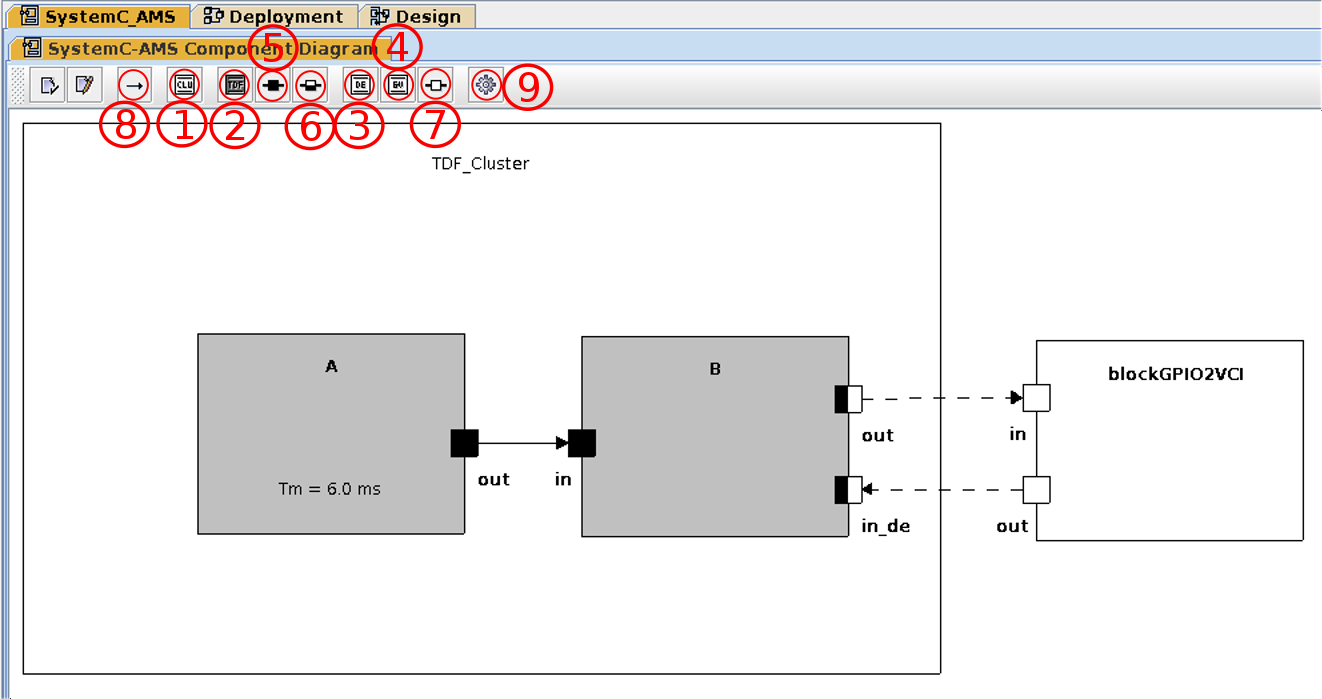
\includegraphics[width=0.7\textwidth]{fig/usage_scenario/tdf_cluster_creation.png}
    \caption{TDF Cluster creation in the SystemC-AMS Component Diagram panel.}
    \label{fig:8.tdf_cluster_creation}
\end{figure}

Inside the SystemC-AMS Component Diagram panel TDF clusters can be created. To create a TDF cluster click on the ``Cluster'' button, number 1 of Figure~\ref{fig:8.tdf_cluster_creation}, and click anywhere inside the SystemC-AMS Component Diagram panel to place the TDF Cluster block. Double-click to change the name of the TDF cluster. The size of the TDF cluster can be adjusted. 

To add TDF module blocks, click on the ``TDF Block'' button, number 2 of Figure~\ref{fig:8.tdf_cluster_creation}, and click anywhere inside the TDF Cluster block to place the TDF Module block. To add a DE module block follow the same procedure, just start by clicking on the ``DE Block'' button, number 3 of Figure~\ref{fig:8.tdf_cluster_creation}. To add a GPIO2VCI block, click on the ``GPIO2VCI block'' button, number 4 of Figure~\ref{fig:8.tdf_cluster_creation}. GPIO2VCI blocks should be placed outside of the TDF Cluster block.


The properties of the TDF module blocks can be set by double-clicking the block. A new window will open, as shown in Figures~\ref{fig:8.block_attributes_window1} to \ref{fig:8.block_attributes_window3}. In the Attributes panel the name and module timestep (Tm) including time units can be set, as Figure~\ref{fig:8.block_attributes_window1} shows. In the Parameters panel, seen in Figure~\ref{fig:8.block_attributes_window2}, the parameters of a TDF module such as its internal variables or template parameters can be also set up. In the Process Code panel, the \texttt{processing()} function of the module can be set, as Figure~\ref{fig:8.block_attributes_window3} shows. Finally, if constructor code needs to be added, it can be done in the Constructor Code panel. The attributes of the DE module blocks can be modified in the same way. The GPIO2VCI block has no attributes to be modified. 

\begin{figure}[h]
    \centering     
         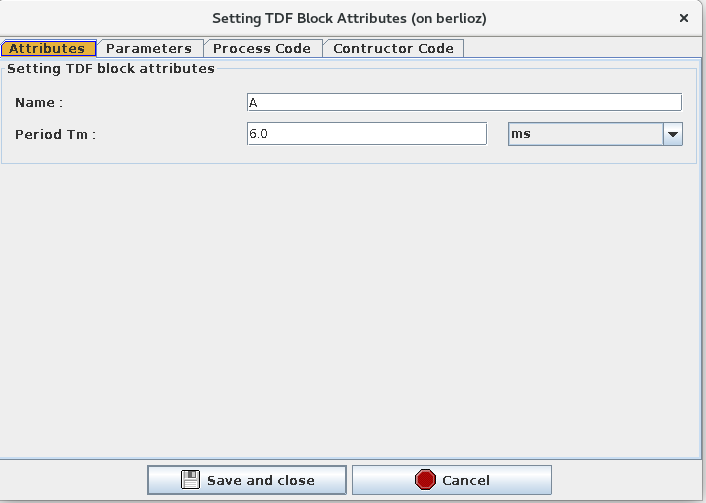
\includegraphics[width=0.6\textwidth, ]{fig/usage_scenario/block_attributes_window1.png}
         \caption{Attributes panel}
         \label{fig:8.block_attributes_window1}
     \end{figure}

  \begin{figure}[h]
         \centering
         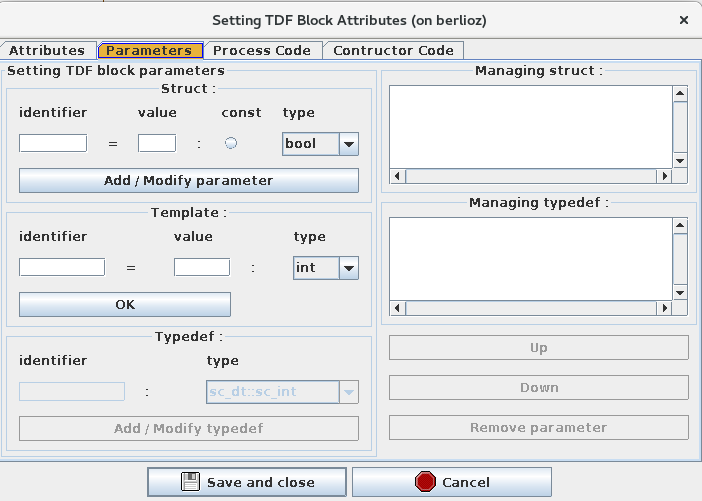
\includegraphics[width=0.6\textwidth, ]{fig/usage_scenario/block_attributes_window2.png}
         \caption{Parameters panel}
         \label{fig:8.block_attributes_window2}
     \end{figure}
    

\begin{figure}[h]
         \centering
         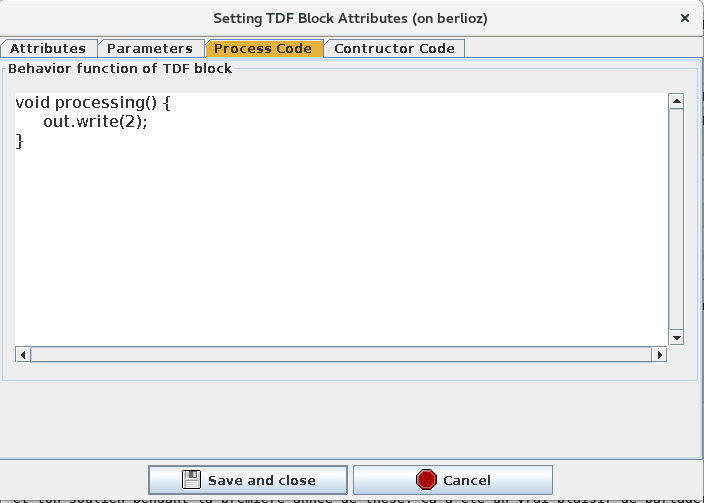
\includegraphics[width=0.6\textwidth, ]{fig/usage_scenario/block_attributes_window3.png}
         \caption{Process Code panel}
         \label{fig:8.block_attributes_window3}
\end{figure}

\begin{figure}[h]
    \centering
    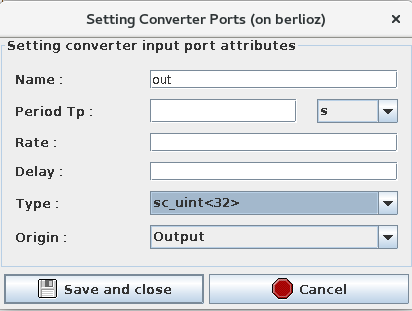
\includegraphics[width=0.45\textwidth]{fig/usage_scenario/port_attributes.png}
    \caption{Setting port attributes.}
    \label{fig:8.port_attributes}
\end{figure}

When the required modules have been created they need to be connected through their ports. The TDF ports and converter ports can be added to the TDF module blocks. Click on the ``TDF port'' button, number 5 of Figure~\ref{fig:8.tdf_cluster_creation}, to add a TDF port. Click on the ``Converter port'' button, number 6 of Figure~\ref{fig:8.tdf_cluster_creation}, to add a TDF converter port. DE ports can be added to the DE blocks and to the GPIO2VCI block by clicking on the DE port button, number 7 of Figure~\ref{fig:8.tdf_cluster_creation}. The attributes of the ports can be modified by double-clicking a port, as shown in Figure~\ref{fig:8.port_attributes}. The name, timestep (Tp) along with the time units, rate, delay, type and origin of the port can be modified. Note that if a TDF module or a DE module will be connected to the GPIO2VCI component, the type \texttt{sc\_uint<32>} should be selected as shown in Figure~\ref{fig:8.port_attributes}.
For DE ports, the port can be added to the sensitivity list of the module by enabling the Sensitive field and selecting if the port will be sensitive to a positive or negative edge of the incoming signal or \texttt{null} for any incoming signal change.
To connect the blocks, click the ``Connector'' button, number 8 of  Figure~\ref{fig:8.tdf_cluster_creation}, and then click an output port to connect it with an input port. 

Once a TDF cluster model has been created. The next step is to validate the correctness of the model. This is done by clicking on the ``Generate SystemC-AMS code'' button, as shown in number 9 from Figure~\ref{fig:8.tdf_cluster_creation}. This will open a new window, where validation of the model and code generation can be made. Click on the ``Start'' button to start the validation of the model, as shown in Figure~\ref{fig:8.validate_model1}. The Validation panel will display a message stating if there is an error with the model and make suggestions on how to fix it. If the model is valid, then a success message will be displayed and the Generate Code panel will open, as shown in Figure~\ref{fig:8.validate_model2}. Click on the ``Start'' button again to generate the SystemC-AMS code for the model. 

\begin{figure}[h]
  
         \centering
         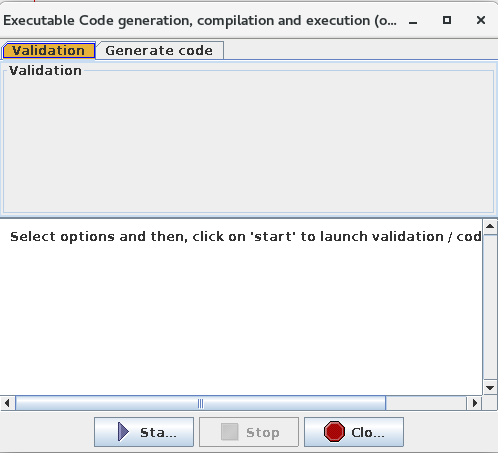
\includegraphics[width=0.6\textwidth]{fig/usage_scenario/validate_model1.png}
         \caption{Validation panel}
         \label{fig:8.validate_model1}
     \end{figure}

\begin{figure}[h]
         \centering
         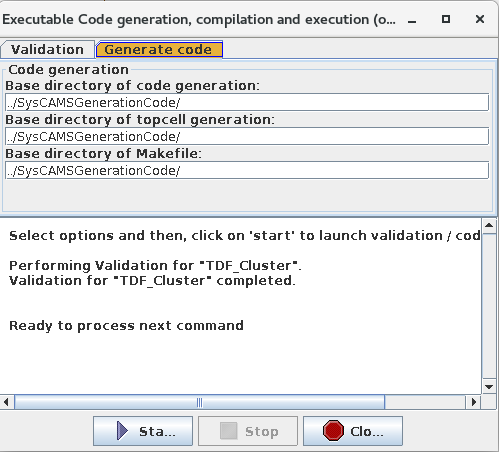
\includegraphics[width=0.6\textwidth]{fig/usage_scenario/validate_model2.png}
         \caption{Generate Code panel}
         \label{fig:8.validate_model2}
     \end{figure}
   
In parallel, the Software Design and the Deployment Diagrams can be created. Right click on the tabs section of the design area and select ``New Design'' to create a new Software Design panel. A Block diagram can be created there, as shown in Figure~\ref{fig:8.usage_scenario_block_diagram}. Click on the ``Block'' button, number 1 of Figure~\ref{fig:8.usage_scenario_block_diagram}, to add a new block. Note that a new panel is created automatically, with the name of the block. Go to the \textbf{Block0} panel. Here, state machine diagrams that allow to design the software can be created, as shown in Figure~\ref{fig:8.usage_scenario_fsm_diagram}. For this model, one state will be added by clicking on the ``State'' button, number 1 of Figure~\ref{fig:8.usage_scenario_fsm_diagram}, and placing it in the panel. 
A stop block can be added by clicking the ``Stop'' button, number 2 of Figure~\ref{fig:8.usage_scenario_fsm_diagram}. Finally the states should be connected by clicking the ``Connect'' button, number 3 of Figure~\ref{fig:8.usage_scenario_fsm_diagram}.

\begin{figure}[h]
    \centering
    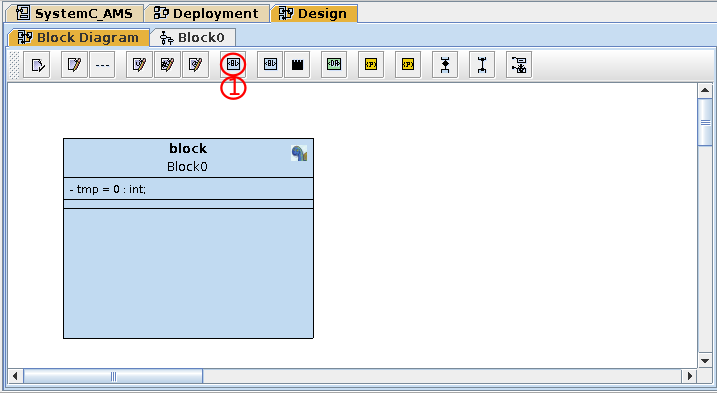
\includegraphics[width=0.6\textwidth]{fig/usage_scenario/usage_scenario_block_diagram.png}
    \caption{Software design Block Diagram panel.}
    \label{fig:8.usage_scenario_block_diagram}
\end{figure}

\begin{figure}[h]
    \centering
    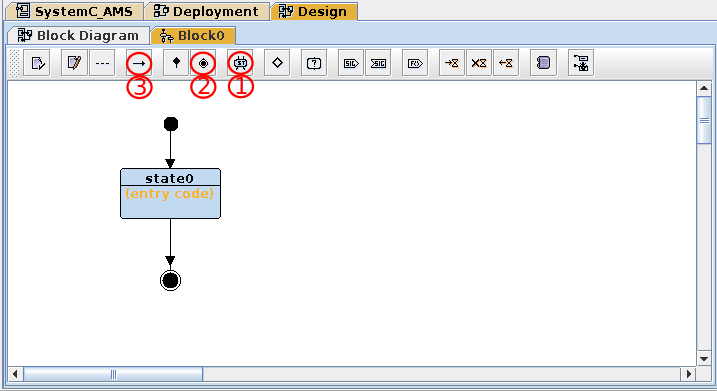
\includegraphics[width=0.6\textwidth]{fig/usage_scenario/usage_scenario_fsm_diagram.png}
    \caption{Software design State Machine Diagram panel.}
    \label{fig:8.usage_scenario_fsm_diagram}
\end{figure}

By double-clicking the state block, C code can be entered manually in the Prototyping tab. Here is where the functions to communicate to the GPIO2VCI component can be added as shown in Figure~\ref{fig:8.usage_scenario_state_block_code}. For the software of this model, a value of 5 will be written to the GPIO2VCI component. This value will be transmitted to the TDF cluster components. Then the output from the TDF cluster will be read and printed to the TTY component of the model. The code is shown in Listing~\ref{code:8.usage_scenario_state_block_code}. 


\begin{figure}[htb]
    \centering
    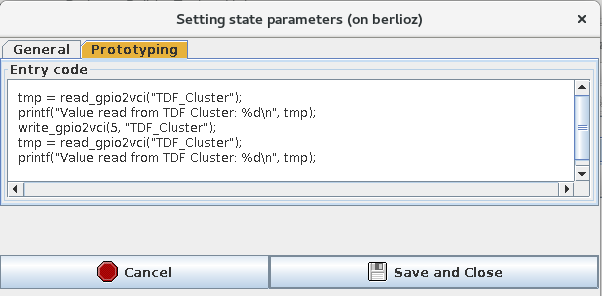
\includegraphics[width=0.45\textwidth]{fig/usage_scenario/usage_scenario_state_block_code.png}
    \caption{State block Prototyping panel .}
    \label{fig:8.usage_scenario_state_block_code}
\end{figure}

\begin{figure}[htb]
\begin{verbatim}
tmp = read_gpio2vci("TDF_Cluster");
printf("Value read from TDF Cluster: %d\n", tmp);
write_gpio2vci(5, "TDF_Cluster");
tmp = read_gpio2vci("TDF_Cluster");
printf("Value read from TDF Cluster: %d\n", tmp);
\end{verbatim}
  \caption{State block code.}
  \label{code:8.usage_scenario_state_block_code}
\end{figure}

Note that the code is using a variable \texttt{tmp}. To create the variable in the Block Diagram panel, double click \textbf{Block0} to open the attributes window for the block, as shown in Figure~\ref{fig:8.block0_attributes}. In the Attributes panel, new variables can be added by giving an identifier name, an initial value and a type.

\begin{figure}[h]
    \centering
    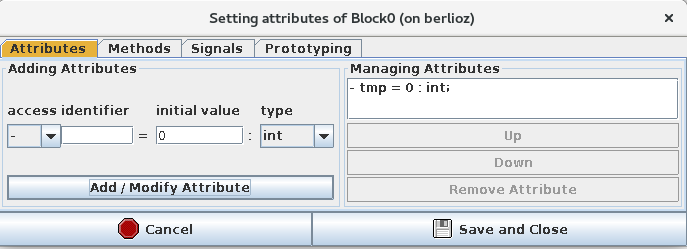
\includegraphics[width=0.45\textwidth]{fig/usage_scenario/block0_attributes.png}
    \caption{Block diagram's Block attributes.}
    \label{fig:8.block0_attributes}
\end{figure}

Once that the software design is complete, the MPSoC model needs to be created in the Deployment Diagram. Here, the user can insert SoCLib components and the TDF clusters. To insert a CPU click the ``CPU'' button, number 1 of Figure~\ref{fig:8.dd_creation}. Double click the CPU block and setup the necessary attributes.
To add a RAM memory click on the ``RAM'' button, number 2 of Figure~\ref{fig:8.dd_creation}. Double click the RAM block and set up its attributes. 
To add a TTY console click on the ``TTY'' button, number 3 of Figure~\ref{fig:8.dd_creation}. Finally an interconnect component needs to be added, by clicking the ``VGMN'' button, number 4 of Figure~\ref{fig:8.dd_creation}. To map the software blocks from the Block Diagram into a specific CPU, click the ``Map and AVATAR block'' button, number 5 of Figure~\ref{fig:8.dd_creation}, and place it under the CPU. Double click the block inside the CPU and select the name of the block that is mapped to that CPU. 


\begin{figure}[h]
         \centering
         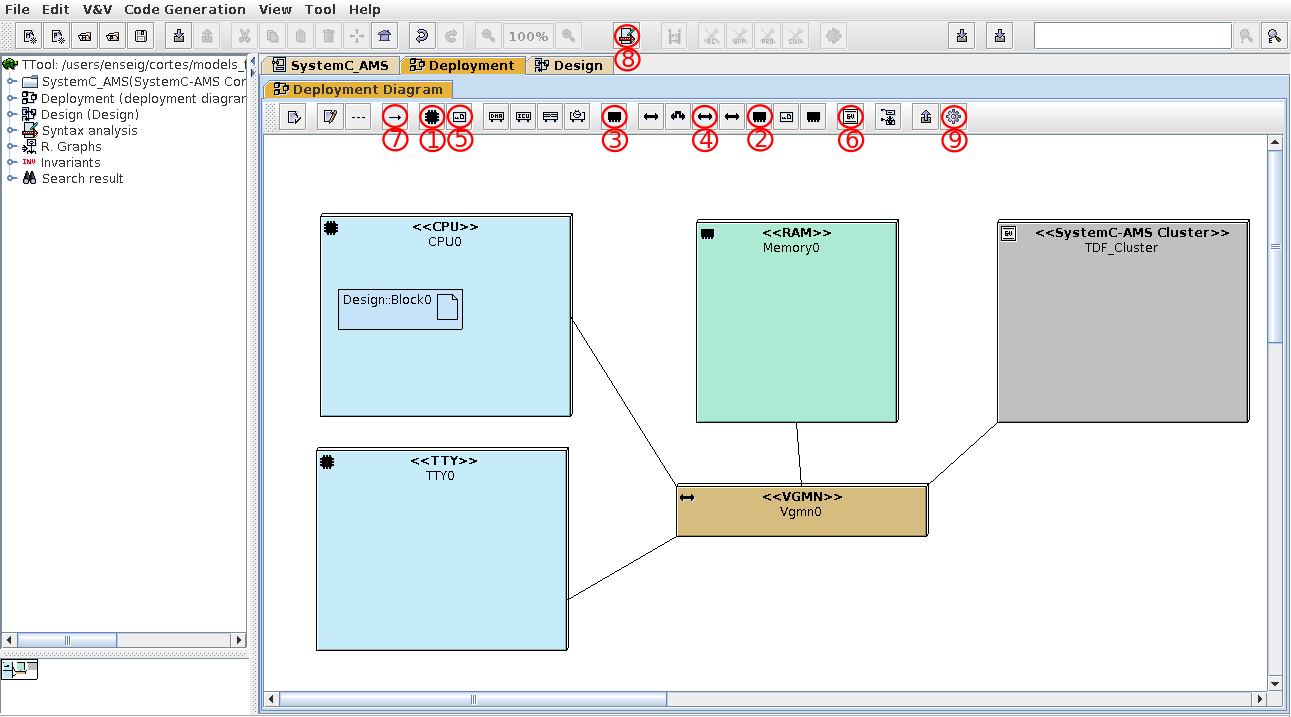
\includegraphics[width=0.85\textwidth]{fig/usage_scenario/dd_creation.png}
         \caption{Adding SystemC-AMS Clusters to the Deployment Diagram.}
         \label{fig:8.dd_creation}
\end{figure}

In order to include the TDF clusters into the MPSoC model, they need to be added as SystemC-AMS Cluster blocks in the Deployment Diagram. To add a new SystemC-AMS Cluster block, click on the ``Cluster'' button, number 6 of Figure~\ref{fig:8.dd_creation}, and place the block in the Deployment Diagram panel. The name of the SystemC-AMS Cluster block should be the same name provided in the SystemC-AMS Component diagram. All the blocks should be connected to a SoCLib interconnect component using a connector, number 7 of Figure~Figure~\ref{fig:8.dd_creation}. Once the necessary SystemC-AMS Cluster blocks have been added, the topcell from the Deployment Diagram model can be generated. In the Deployment Diagram Panel, click on the ``Syntax analysis'' button, number 8 of Figure~\ref{fig:8.dd_creation}. This will open a new window to verify the syntax of the model, as shown in Figure~\ref{fig:8.dd_syntax}. Click on the ``Check syntax'' button. If there are any syntax errors, a message will be displayed, otherwise we can proceed to the generation of the topcell. 

\begin{figure}[h]
         \centering
         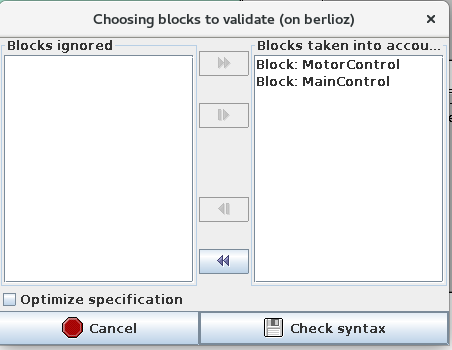
\includegraphics[width=0.5\textwidth]{fig/usage_scenario/dd_syntax.png}
         \caption{Check syntax window.}
         \label{fig:8.dd_syntax}
\end{figure}

\begin{figure}[H]
         \centering
         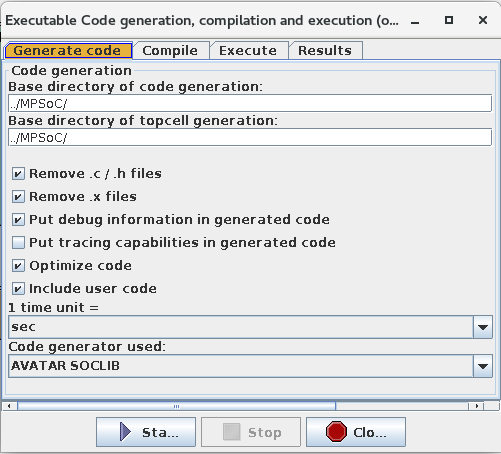
\includegraphics[width=0.5\textwidth]{fig/usage_scenario/topcell_code_generation1.png}
         \caption{Code generation window.}
         \label{fig:8.topcell_code_generation1}
\end{figure}

Click on the ``Generate Deploy SoCLib'' button in the Deployment Diagram panel, number 9 of Figure~\ref{fig:8.dd_creation}. A new window will be opened where the topcell code can be generated, compiled and executed. In Figure~\ref{fig:8.topcell_code_generation1}, the Generate Code panel is shown, where several option can be chosen, including the tracing capabilities and debugging information. Click ``Start'' to generate the topcell \texttt{top.cc} code and the software code. Then in the Compile panel, click ``Start'' to compile the code. Finally in the Execute panel, click ``Start'' to begin the simulation of the virtual prototype of the model.

Figure~\ref{fig:8.model_sim_output} shows the TTY console from the model. In the last lines, the values being read from the TDF cluster are printed. The first value is 0, since nothing have been written to the TDF cluster. The last value is 10, since a value of 5 was written to the TDF cluster, and it is being multiplied by the value 2 generated from the TDF module \textbf{A}.
\begin{figure}[H]
         \centering
         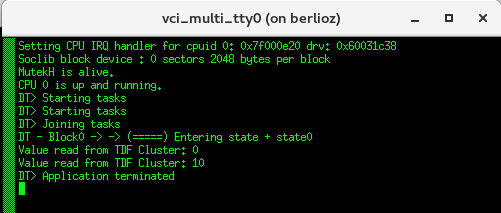
\includegraphics[width=0.7\textwidth]{fig/usage_scenario/model_sim_output.png}
         \caption{Simulation output from the TTY component of the model.}
         \label{fig:8.model_sim_output}
\end{figure}



\newpage
\clearpage
\section{Directory tree of source code and generated files}
\label{sec:appendix-dir-tree}

In this section, the directory tree of all source files modified for this project and all the generated files is shown. Listing~\ref{tree:generated_source_code} shows the location of the automatically generated files from TTool. The SystemC-AMS generated files for the TDF clusters are stored under the \texttt{generated\_CPP/} directory, and the generated files for the TDF modules are stored under the \texttt{generated\_H/} directory. The generated source code files for the software of the virtual prototype are stored under the \texttt{generated\_src/} directory. The generated topcell is stored in the \texttt{generated\_topcell/} directory.

\begin{figure}[h]
\dirtree{%
.1 \$HOME/TTool/.
.2 SysCAMSGenerationCode/.
.3 generated\_CPP/.
.4 *\_tdf.h.
.3 generated\_H/.
.4 *\_tdf.h.
.2 MPSoC/.
.3 generated\_src/.
.4 main.c.
.4 Block0.c.
.3 generated\_topcell/.
.4 top.cc.
}
  \caption{Generated code files directories.}
  \label{tree:generated_source_code}
\end{figure}

The GPIO2VCI component was created under the \texttt{connectivity\_component/} directory, as shown in Listing~\ref{tree:gpio2vci_dir}

\begin{figure}[h]
\dirtree{%
.1 \$HOME/TTool/MPSoC/soclib/soclib/module/connectivity\_component/gpio2vci/caba/.
.2 metadata/.
.3 gpio2vci.sd.
.3 source/include/.
.4 gpio2vci.h.
.3 source/src/.
.4 gpio2vci.cpp.
}
  \caption{GPIO2VCI component directories.}
  \label{tree:gpio2vci_dir}
\end{figure}

\newpage
Listing~\ref{tree:ttool_java_files} shows the java files that were modified or created as part of the integration of the SystemC-AMS modules and SoCLib modules into TTool.

\begin{figure}[htb]
\dirtree{%
.1 \$HOME/TTool/src/main/java/.
.2 ui/.
.3 window/.
.4 JDialogSysCAMSExecutableCodeGeneration.java.
.4 JDialogSysCAMSBlockDE.java.
.4 JDialogSysCAMSBlockTDF.java.
.4 JDialogSysCAMSPortConverter.java.
.4 JDialogSysCAMSPortDE.java.
.4 JDialogSysCAMSPortTDF.java.
.3 AvatarDeploymentPanelTranslator.java.
.2 syscamstranslator/.
.3 toSysCAMSCluster/.
.4 ClusterCode.java.
.4 Header.java.
.4 PrimitiveCode.java.
.4 TopCellGeneratorCluster.java.
.3 SysCAMSTBlockTDF.java.
.3 SysCAMSSpecification.java.
.3 SysCAMSTPortDE.java.
.3 SysCAMSTPortTDF.java.
.3 SysCAMSTPortConverter.java.
.3 SysCAMSValidateException.java.
.2 ddtranslatorSoclib/.
.3 toSoclib/.
.4 Gpio2VciAddress.java.
.4 TaskFileSoclib.java.
.4 TasksAndMainGenerator.java.
.3 toTopCell/.
.4 Declaration.java.
.4 Header.java.
.4 MappingTable.java.
.4 NetList.java.
.4 Platforminfo.java.
.4 Signal.java.
.4 TopCellGenerator.java.
.3 AvatarAmsCluster.java.
.3 AvatarddSpecification.java.
}
  \caption{Java files created or modified for the integration of SystemC-AMS and SoCLib modules.}
  \label{tree:ttool_java_files}
\end{figure}

\newpage
The \texttt{libsyscams} library created to provide interface functions for communication with the GPIO2VCI component is shown under Listing~\ref{tree:libsyscams}.

\begin{figure}[htb]
\dirtree{%
.1 \$HOME/TTool/MPSoC/mutekh/libsyscams/.
.2 gpio2vci\_address.c.
.2 gpio2vci\_address.h.
.2 gpio2vci\_iface.c.
.2 gpio2vci\_iface.h.
.2 libsyscams.config.
.2 Makefile.
}
  \caption{\texttt{libsyscams} library source files.}
  \label{tree:libsyscams}
\end{figure}

Listing~\ref{tree:other_files} shows other files that were modified as part of the integration tasks.

\begin{figure}[H]
\dirtree{%
.1 \$HOME/TTool/MPSoC/.
.2 Makefile.forsoclib.
.2 generated\_topcell/.
.3 config\_noproc.
}
  \caption{Other modified files for the integration tasks.}
  \label{tree:other_files}
\end{figure}


%%%%%%%%%%%%%%%%%%%%%%%%%%%%%%%%%}}}%
\end{document}
